\section{Einleitung}
Dieses Dokument ist ein Teil der Dokumentation des Projektes Imager-Emu\-lator. Dieses Projekt besteht aus drei Teilprojekten. 
Genauer gesagt besteht es aus zwei Bachelor-Thesen und einem Projekt 5 (P5) des Studienganges Elektro- und Informationstechnik der Fachhochschule Nordwestschweiz. 
Das P5 und die erste Thesis laufen parallel, die zweite Thesis wird ein Semester später durchgeführt. Die vorliegende Dokumentation ist diejenige von der ersten Thesis, welche parallel mit dem Projekt 5 durchgeführt wird. Das Projekt 5 und die zweite Thesis wird von Fabio Nardo geschrieben und diese Dokumentation ist von mir, Marc de Bever, geschrieben. 

Das Projekt Imager-Emulator wurde von der Firma Varian Medical Systems ausgeschrieben. Das Ziel is es, einen Röntgensensor zu emulieren. Der Sensor wird auch Imager genannt, wenn die ganze zugehörige Elektronik gemeint ist. Daher kommt der Name Imager-Emulator. Der Sensor gibt Bilder über eine nicht standardisierte Schnittstelle an einen Computer weiter. Der Computer, welcher die Bilder des Sensors entgegen nimmt, rechnet diverse Algorithmen, die unteranderem Pixelfehler erkennen und korrigieren. Jedoch kann dem Sensor nicht gesagt werden, \textit{mach mal 'nen Pixelfehler}. Daher braucht es ein Hardware-Emulator, um Bilder mit Pixelfehlern zu generieren und an den Computer zu senden. Mit Hilfe von diesem Emulator können die Algorithmen des Computers in einem realitätsnahen System getestet werden. Der Emulator soll über USB Konfiguriert werden. Somit ergibt sich das Blockdiagramm in Abbildung \ref{fig:bd_sehr_grob}. Ein Computer konfiguriert den Emulator über USB, dieser gibt sich als Imager aus und überträgt die gewünschten Bilder mit den Pixelfehlern auf den XI-Computer. Der XI-Computer ist der Computer, auf dem die Algorithmen laufen. Um die Algorithmen zu testen, bekommt der Computer via Ethernet die berechneten Bilder wiederum  und kann diese mit den erwarteten Bilder verglichen.

\begin{figure}[H]
    \centering
    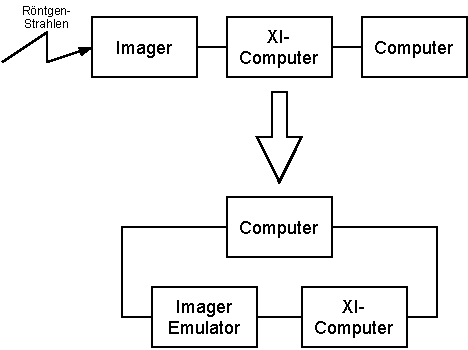
\includegraphics[width=0.6\linewidth]{bd_sehr_grob}
    \caption{Überblick über das Projekt}
    \label{fig:bd_sehr_grob}
\end{figure}

Da dieses Projekt eine spezielle Konstellation hat, ist die Aufteilung der Teilprojekte wie folgt:
\begin{itemize}
\item Das P5 soll die Hardware entwickeln. 
\item Die erste Thesis, also diese Arbeit, soll die Entwicklungsumgebungen und das FPGA-Modul in Betrieb genehmen, sowie auch die Schnittstellen programmieren. 
\item Die zweite Thesis soll schlussendlich die Kommunikation mit dem Computer implementieren, es ermöglichen Pixelfehler in die Bilder einzubauen und das ganze Projekt abzuschliessen.
\end{itemize}

Dieser Bericht dient zum einen dazu, dass im weiterführenden Projekt verstanden wird, wie die Entwicklungsumgebung und Schnittstellen funktionieren, wo deren Möglichkeiten und Grenzen liegen, und zum anderen dient er, um diese Arbeit als Thesis zu dokumentieren. Der Bericht ist folgendermassen aufgebaut.

Das zweite Kapitel beschreibt wie das Projekt konzeptuell aufgebaut ist. Dafür beschreibt es das Projekt mit drei verschiedenen Systemen. Als erstes das, welches von der Varian schon vorhanden ist. Dieses soll durch dieses Projekt emuliert werden. Das zweite System ist eine Zwischenlösung, damit gleichzeitig die Hardware und die Software entwickelt werden kann. Und das letzte System ist das endgültige Gerät, welches den Sensor der Varian emuliert. Diese Kapitel soll einen Top-Down-Blick auf das Projekt geben. Zusätzlich beschreibt es die Wahl der wichtigsten Komponente, des FPGA-Moduls.

Das dritte Kapitel beschreibt den geschrieben Code. Jener besteht aus zwei Teilen, der Firmware für den Mikrocontroller und der für den FPGA. Dieses Kapitel erwähnt zum Teil Sachen des zweiten Kapitels nocheinmal. Aber anstatt einen Überblick zu geben, soll dieses Kapitel sich auf die Details konzentrieren.

Das vierte Kapitel beschreibt wie der Imager-Emulator konfiguriert wird und wie zusätzliche Konfigurationen nachträglich hinzugefügt werden können.

Und zu guter Letzt, das fünfte Kapitel beschreibt die Entwicklungsumgebungen (IDEs), mit welchen der Code entwickelt wurde. Dieses Kapitel beschreibt zuerst wie diese aufgebaut sind, was sie können und wie sie zusammenhängen. Als nächstes wird beschrieben, wie man mit den IDEs die Hardware debuggen kann und als letztes die Grenzen der Entwicklungsumgebungen.